\section{Other tools and algorithms}
\subsection*{Adaptable moment estimation (ADAM) Optimizer}
Stochastic gradient descent, though very useful, lack the ability to adapt to the feature space. One algorithm that address this
issue is the ADAM optimizer\cite{ADAM:opti}. The Adaptable moment estimation (ADAM) algorithm uses stochastic gradient descent, but with 
an adaptiv learning rate. This learning rate is adjusted by calculating estimates for the first and second moment\footnote{In statistics
the first moment is the expectation value for a distribution, $E[X-\mu]$. The second moment is the 
expectation value of the distribution squared, i.e the variance, $E[(X-\mu)^2]$}. Thus, a large gradient would indicate close proximity 
to a minimum in feature space, thus a lower learning rate would yield a more accurate result, 
where as a small gradient would suggest far proximity to a local minimum, and thus a larger learning rate would increase the chance 
of approaching a minimum.\par 

\subsection*{Hyperband}
Hyperband is a tool for hyperparameter optimization\cite{hyperband:opt}. Hyperparameter optimization is of high importance in the 
search for ideal structures and architectures when using neural networks, as there is not a way to find an a priori setup for a 
given problem. Several algorithms are used, from random search, grid search, and bayesian optimization. Hyperband is an algorithm 
proposed by L. Li et al. It focuses on using successful halving\cite{successivehalving}
but at the same time doing a grid search for how to allocate resources. Successive halving focuses on testing n configurations, and removing 
the bottom half, thus (hopefully) quickly converging to the ideal combination. However, it is not easy to a priori know the 
number of configurations n, and how many resources one needs, r, to quickly find the ideal set. This is where Hyperband comes in. 
In essence, it fetches and tries different combinations of r resources (time, data set subsampling or feature subsampling) and n 
configurations, to determine the ideal set of hyperparameters via successive halving, yielding 5x to 30x speedup compared to 
Bayesian optimization. One drawback for this algorithm is that one cannot guarantee that the configuration is optimal, 
but rather that it is only good enough. 

\subsection*{Activation functions}
Several activation functions are used in neural networks, and how one chooses the best combination for a given problem is not trivial. 
This often leads to the use of tuning. Below are a list of the activation functions used in this thesis, and their mathematical definitions. 

\begin{enumerate}
    \item  $sigmoid(x) = \frac{1}{1+e^{-x}}$
    \item $tanh(x) = \frac{e^x-e^{-x}}{e^x+e^{-x}}$
    \item $ReLU(x) = \max(0,x)$
    \item $LeakyReLU(x) = \max(\alpha x,x)$
    \item $Softmax(x) = \frac{e^x}{\sum_{i=1}^n e^x}$
    \item $Linear(x) = x$
\end{enumerate}


\subsection*{ROC curve}
One way to measure the effectiveness of a prediction for a machine learning algorithm is with the use of a ROC curve. 
The ROC curve is a plot of the true positive rate (TPR) against the false positive rate (FPR) which will be defined shortly. 
Suppose a classifier $\mathcal{M}$ does a binary classification of positive and negative. If $\mathcal{M}$ predicts a positive 
label, and the instance is indeed positive, we define this as a $\it{true\, positive}$. The same goes for negative prediction of a 
negative instance, which is defined as a $\it{true\, negative}$. Then there is the case where $\mathcal{M}$ predicts a negative label
when the instance is positive, defined as a $\it{false\, negative}$, and vice versa is then defined as a $\it{false\, positive}$\cite{FAWCETT2006861}.
Now, the TPR is defined as the ratio of true positives to the total number of positive instances, i.e. 
\begin{equation*}
    TPR = \frac{TP}{TP+FN},
\end{equation*}
and the FPR is defined as the ratio of false positives to the total number of negative instances, i.e.
\begin{equation*}
    FPR = \frac{FP}{FP+TN}.
\end{equation*}
Using this, we get a plot that tells us how well the classifier performs. As the goal is usually to have a high TPR and a low FPR,
the more "north-west"\cite{FAWCETT2006861} of the plot the curve is, the better. Below are two example of a ROC curve and the classifier output it 
is calculated from. For simplicity, the classifier output is in this case just two normal distributions with the mean and standard deviation 
listed in the legend of the distribution plots.
\marginpar{Bytt "here we get" med "the"}
\begin{figure}[H]
    \centering
    \begin{subfigure}{.45\textwidth}
        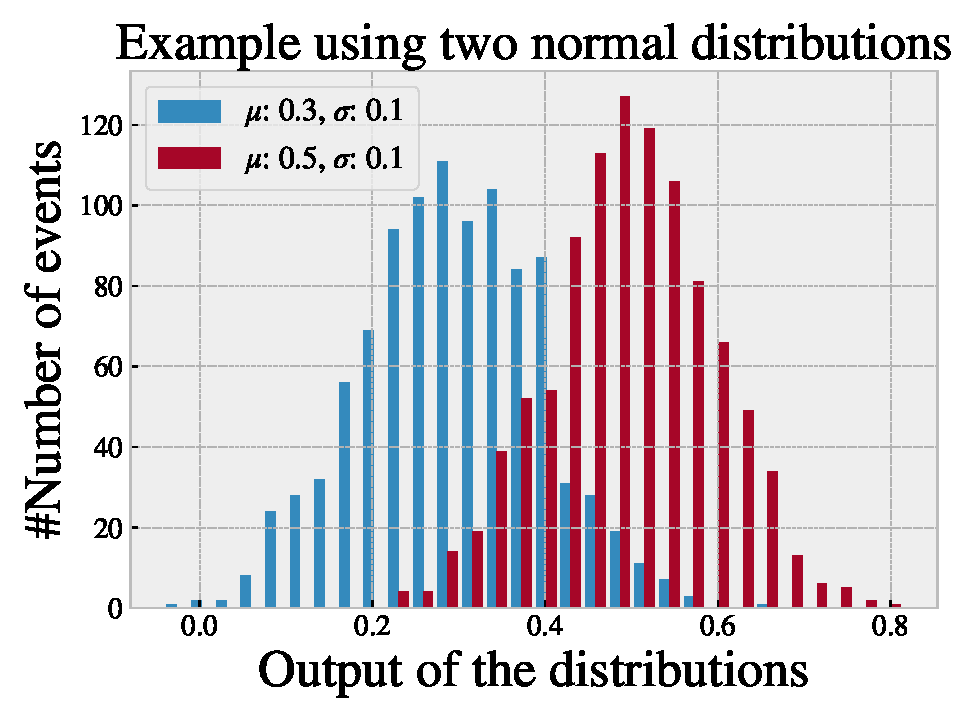
\includegraphics[width=\textwidth]{Figures/Machinelearning/histo_example_Sep.pdf}
        \caption{Histogram showing good separation. Here the left distribution is calculated using a mean of 0.3 and a standard 
        deviation of 0.1, and the right distribution is calculated using a mean of 0.5 and a standard deviation of 0.1.}
        \label{fig:dist_ex_good}
    \end{subfigure}
    \hfill
    \begin{subfigure}{.45\textwidth}
        \includegraphics[width=\textwidth]{Figures/Machinelearning/ROC_curve_example_Sep.pdf}
        \caption{ROC curve based on the two distributions to the left. The area under the curve score of 0.92, which is very good. }
        \label{fig:ROC_curve_ex_good}
    \end{subfigure}
    \hfill        
    \caption{Histogram and ROC curve for two well separated distributions.}
    \label{fig:roc_example_good}
\end{figure}

\begin{figure}[H]
    \centering
    \begin{subfigure}{.45\textwidth}
        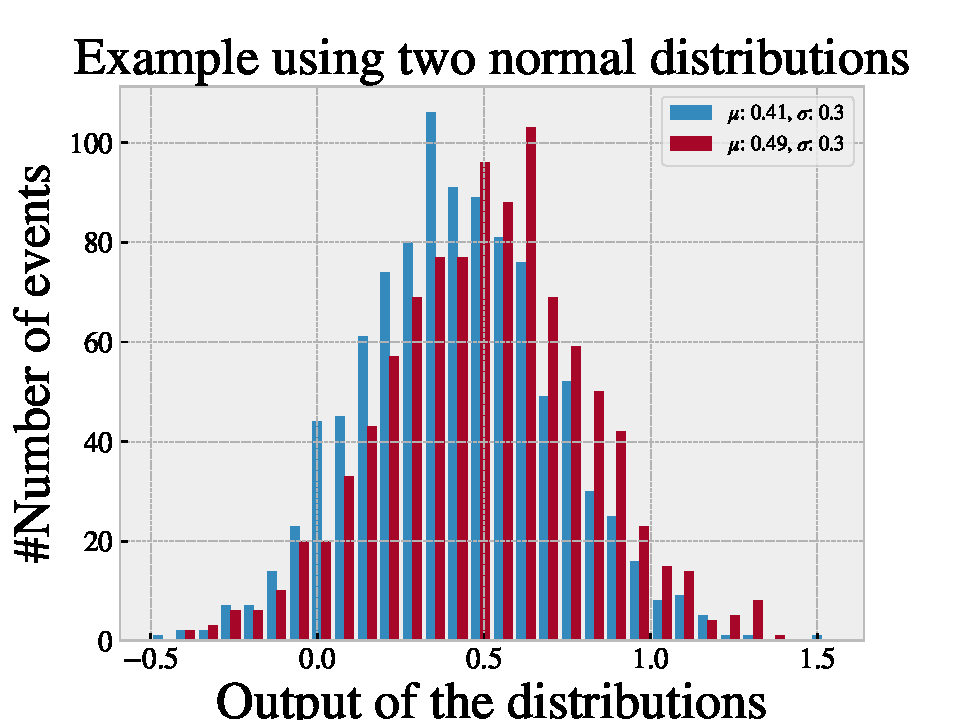
\includegraphics[width=\textwidth]{Figures/Machinelearning/histo_example_bad.pdf}
        \caption{Histogram showing bad separation. Here the left distribution is calculated using a mean of 0.41 and a standard 
        deviation of 0.3, and the right distribution is calculated using a mean of 0.49 and a standard deviation of 0.3.}
        \label{fig:dist_ex_bad}
    \end{subfigure}
    \hfill
    \begin{subfigure}{.45\textwidth}
        \includegraphics[width=\textwidth]{Figures/Machinelearning/ROC_curve_example_bad.pdf}
        \caption{ROC curve based on the two distributions to the left. The area under the curve score of 0.58, which is not a good classification score.}
        \label{fig:ROC_curve_ex_bad}
    \end{subfigure}
    \hfill        
    \caption{Histogram and ROC curve for two poorly separated distributions.}
    \label{fig:roc_example_bad}
\end{figure}

In figure \ref{fig:roc_example_good} we have a histogram showing two distributions that are well separated, and the ROC curve that is calculated 
based on those distributions. If we compare this to figure \ref{fig:roc_example_bad}, we see that the better separation of the two distributions, the better ROC curve. 
This is a useful tool to use with the autoencoder as it provides valueable insight beyond just looking at the output distributions. \marginpar{More info?}

\subsection*{Statistical significance}
In the frequentist statistics, the Poisson distribution can be approximated with a Gaussian distribution in the limit of large number of events\cite{magnar}. 
The expression for the significance is given then as 
\begin{equation}\label{eq:significance_large}
    Z = \frac{s}{\sqrt{b}},
\end{equation}
where s is the amount of signal, and b is the amount of background. For low statistics we have that the significance is given as 
\begin{equation}\label{eq:significance_small}
    Z = \sqrt{2\left[(s+b)\ln(1+\frac{s}{b})-s\right]}.
\end{equation}
It can be shown that in the limit where $s << b$, the two expressions are approimately the same\cite{magnar}.

\marginpar{More on chapter 1?}